\documentclass[12,french]{report} 
\usepackage{geometry}
\geometry{vmargin=3cm, hmargin=3cm}
\usepackage[T1]{fontenc}
\usepackage[utf8]{inputenc}
\usepackage[french]{babel}
\usepackage{graphicx}
\usepackage{amsmath}
\usepackage{amssymb}
\usepackage{sectsty}
\usepackage{authblk}
\usepackage{algpseudocode}
\usepackage{algorithm}
\usepackage{xspace}
\usepackage{mathtools}
\usepackage{mathrsfs}
\usepackage{enumitem}
\usepackage{titlesec}
\usepackage{hyperref}
\usepackage{xcolor}
\usepackage[justification=centering]{caption}
\usepackage{float}
\usepackage{tabto}

\usepackage{listings}
\usepackage{cleveref}

\renewcommand{\lstlistingname}{Code}
%\renewcommand{\figurename}{Fig.}

\lstdefinestyle{chstyle}{%
backgroundcolor=\color{gray!12},
basicstyle=\ttfamily\small,
showstringspaces=false,
numbers=left}

%\AddThinSpaceBeforeFootnotes
%\FrenchFootnotes

\titleformat{\chapter}[hang]{\bf\Huge}{\thechapter.}{2pc}{}
\titlespacing*{\chapter}{10pt}{0pt}{40pt}[0pt]
\newcommand{\HRule}{\rule{\linewidth}{0.5mm}}

\providecommand{\keywords}[1]{\textbf{\textit{Keywords:}} #1}
\bibliographystyle{apalike}

\usepackage{hyperref}

\begin{document}
\hypersetup{pdfborder=0 0 0}

\begin{titlepage}

\begin{center}
	\vspace*{\stretch{1}}
	\textsc{\LARGE Institut national des sciences appliquées de Rouen} 
	\vspace{5mm}\\
	
\includegraphics[width=0.4\textwidth]{./Images/insa}\\[1.0 cm]

	\textsc{\Large Projet MMSN GM3 - Vague 3 - Sujet 4}\\[0.6cm]

	% Title
	\HRule \\[0.5cm]
	{ \Huge \bfseries Etude des erreurs sur la méthode du Gradient Conjugué}\\[0.2cm]
	\HRule \\[0.75cm]

	
\includegraphics[width=0.6\textwidth]{./Images/Page_de_garde}\\[0.9 cm]

	% Author and supervisor
	\begin{minipage}{0.4\textwidth}
		\begin{flushleft} \large
			\emph{Auteurs:}\\
			Thibaut \textsc{André-Gallis} \\
			{\small\href{mailto:thibaut.andregallis@insa-rouen.fr}{thibaut.andregallis@insa-rouen.fr}} \\
			Kévin \textsc{Gatel} \\
			{\small\href{mailto:kevin.gatel@insa-rouen.fr}{kevin.gatel@insa-				rouen.fr}}
		\end{flushleft}
	\end{minipage}
	\begin{minipage}{0.4\textwidth}
		\begin{flushright} \large
			\emph{Enseignants:} \\
			Bernard \textsc{Gleyse} \\
			{\small\href{mailto:bernard.gleyse@insa-rouen.fr}								{bernard.gleyse@insa-rouen.fr}}\\
		\end{flushright}
	\end{minipage}
	\vspace*{\stretch{1}}

	\vfill
	{\large 6 Juin 2021}
\end{center}
\end{titlepage}

\tableofcontents

%\listoffigures

\renewcommand{\chaptername}{}
\chapter*{Introduction} %thib
\addcontentsline{toc}{chapter}{Introduction}
Pour commencer, nous avons longtemps pensé que les calculatrices et les ordinateurs étaient les références absolues en termes de calcul mathématique. Qu'ils ne se trompaient jamais pourvu qu'on leur donne le bon calcul. Cependant nous avons par la suite découvert que les réels n'existaient pas en machine et qu'on utilisait les flottants pour les représenter. Nous ne détaillerons pas la construction des flottants, ce n'est pas notre sujet mais il est important de connaître leur existence. De cela nous avons compris qu'il était impossible de représenter tous les réels par les flottants. Ce qui entrainera forcément des erreurs inévitables lors des calculs. \\

C'est là tout le sujet de notre projet, les erreurs. En effet nous allons nous intéresser aux erreurs de calculs survenus lors de la résolution d'un système linéaire sur machine. Plus particulièrement avec la méthode du gradient conjugué que nous avons déjà étudié auparavant lors d'un précédent projet. Nous allons donc à l'aide de la valeur binaire des nombres et de la connaissance de la construction des flottants pouvoir étudier et quantifier les erreurs survenues lors de la résolution du système linéaire. \\

Pour obtenir une étude plus large tous les calculs ont été réalisés sur deux machines différentes dont les caractéristiques ont été détaillés dans le fichier "README". Nous pourrons par conséquent les comparer pour remarquer des éventuelles différences d'une machine à l'autre.

\chapter{Présentation du problème} %kev

L'objectif est donc d'étudier les erreurs que fait la machine en utilisant l'arithmétique flottante plutôt que l'ensemble théorique des réels.\\

 Ces erreurs seront étudiées sur la solution du problème linéaire $Ax=b$ avec la méthode du gradient conjugué. En choisissant la matrice $A$ de dimension 4 définie comme ci-dessous :\\

\begin{figure}[H]
	\center
	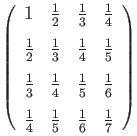
\includegraphics[width=0.2\textwidth]{./Images/H_4}
	\caption{Matrice de Hilbert de dimension 4}
\end{figure}

Le nombre d'étape pour trouver la solution sera en théorie inférieur ou égale à 4 (assuré par la méthode du gradient conjugué).\\

En notant $K_2(A)$ le conditionnement 2 de A tel que :\footnote{conditionnement obtenu sur Matlab}
$$K_2(a)= 1.5514*10^4$$

On a l'inégalité du conditionnement pour majorer l'erreur :
$$\frac{||\Delta x||_{2}}{||x||_2}\leq K_2(A)\frac{||\Delta b||_{2}}{||b||_2}$$

Le test d'arrêt est de la forme $$tol^2*(b,b) > (r,r) $$
avec $(\bullet,\bullet)$ le produit scalaire usuel et $tol=10^{-10}$.\\

Enfin, le vecteur $b$ est choisi comme ci-dessous :

$$b_i=\sum_{k=1}^4A_{ik}$$

de manière à avoir 
$$x^T=\left(\begin{array}{cccc}
1 & 1 & 1 & 1\end{array}\right)$$




\chapter{Vecteur résidu $r$} %thib

\section{Préambule}

Premier élément d'intérêt de notre projet, le vecteur résidu. Intéressons nous aux erreurs faites par la machine sur ce vecteur. Nous ne reviendrons pas sur le rôle du vecteur résidu dans la méthode du gradient conjugué mais il est essentiel au bon fonctionnement de celle-ci.\\
Maintenant nous allons expliquer la démarche utilisée pour étudier cette erreur.

\begin{figure}[H]
	\center
	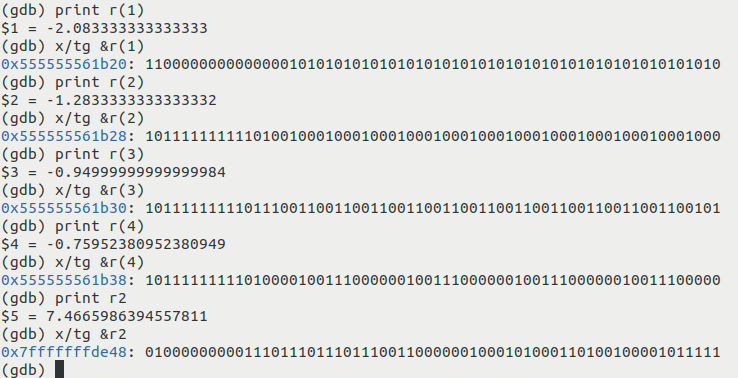
\includegraphics[width=1\textwidth]{./Images/Exemple_gdb}
	\caption{Capture d'écran avec le logiciel gdb}
\end{figure}

Comme on peut le voir ci-dessus, nous avons utilisé le logiciel gdb avec notre programme de gradient conjugué. On utilise le logiciel gdb pour obtenir certaines valeurs pendant le déroulement du programme et pas uniquement à la fin. En ce qui nous concerne nous récupérons les valeurs des composantes du vecteur résidu ainsi que leurs valeurs binaires qui seront importantes pour la suite. la composante r2 est la norme 2 au carré du vecteur résidu et c'est précisément ce que nous allons comparer avec notre calcul pour trouver l'erreur.\\

\begin{figure}[H]
	\center
	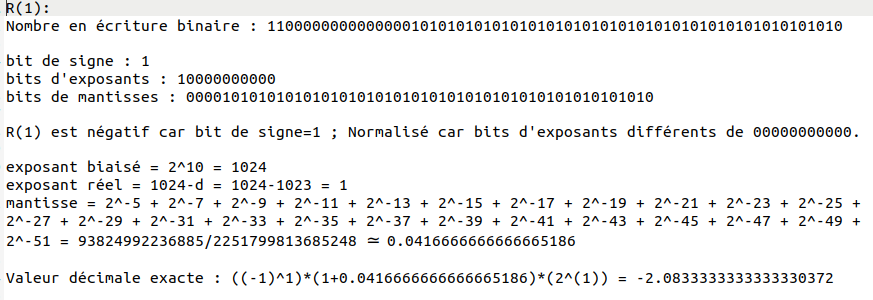
\includegraphics[width=1\textwidth]{./Images/r_0_dec}
	\caption{Conversion binaire réel}
\end{figure}

Deuxième étape, on retrouve la valeur réel en base 10 de notre nombre à partir de son écriture binaire en flottant.\\
On décompose le nombre par bits de signes, exposants et mantisses. On recalcule chacun des termes puis la valeur réelle finale grâce au logiciel en ligne wolframalpha. \\
Maintenant que nous avons la valeur réelle de chaque composante nous allons pouvoir en déduire une valeur calculée par nous même de r2 et la comparé avec celle donnée par l'ordinateur.\\
C'est ce que nous allons maintenant voir à chaque étape de l'itération du gradient conjugué et observé l'erreur absolue et relative entre la solution de l'ordinateur et la notre.


\section{Etape 0}

\begin{figure}[H]
	\center
	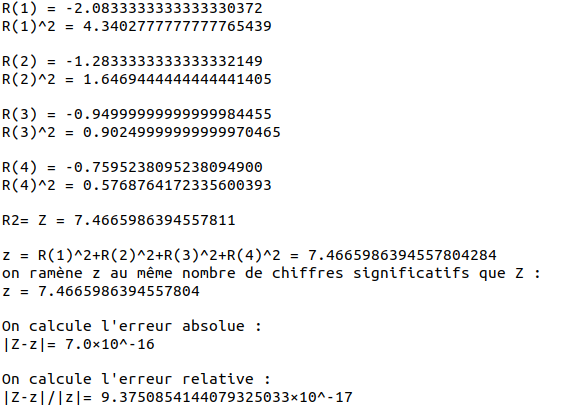
\includegraphics[width=0.9\textwidth]{./Images/r_0_err}
	\caption{Fichier d'erreur à l'étape 0}
\end{figure}

On peut voir que l'erreur absolue est de $10^{-16}$ et l'erreur relative de $10^{-17}$. On est autour de la précision machine pour un double précision et l'erreur relative reste extrêmement faible. On peut être plutôt satisfait du résultat.

\section{Etape 1}

\begin{figure}[H]
	\center
	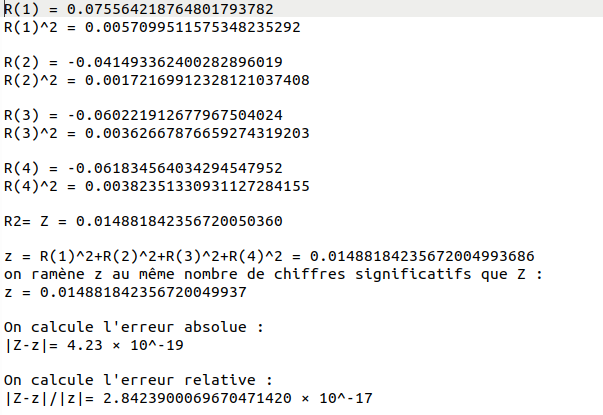
\includegraphics[width=0.9\textwidth]{./Images/r_1_err}
	\caption{Fichier d'erreur à l'étape 1}
\end{figure}

Cette fois l'erreur absolue est de $10^{-19}$ et la relative de $10^{-17}$ c'est même moins que l'étape d'avant.

\section{Etape 2}

\begin{figure}[H]
	\center
	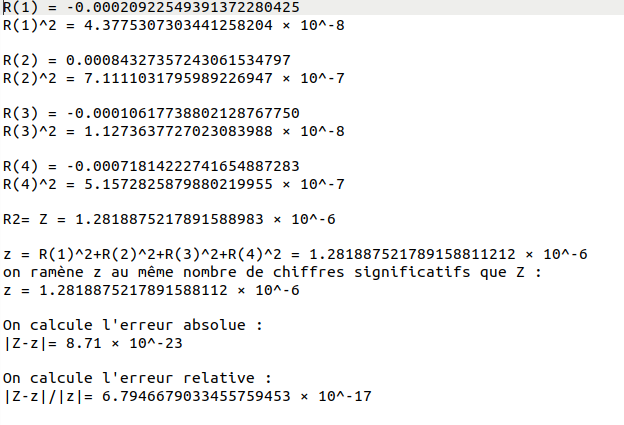
\includegraphics[width=0.9\textwidth]{./Images/r_2_err}
	\caption{Fichier d'erreur à l'étape 2}
\end{figure}

Une fois de plus l'erreur absolue diminue elle est de $10^-{-23}$ cependant quand on regarde l'erreur relative en $10^{-17}$ on se rend compte qu'elle na pas diminué.

\section{Etape 3}

\begin{figure}[H]
	\center
	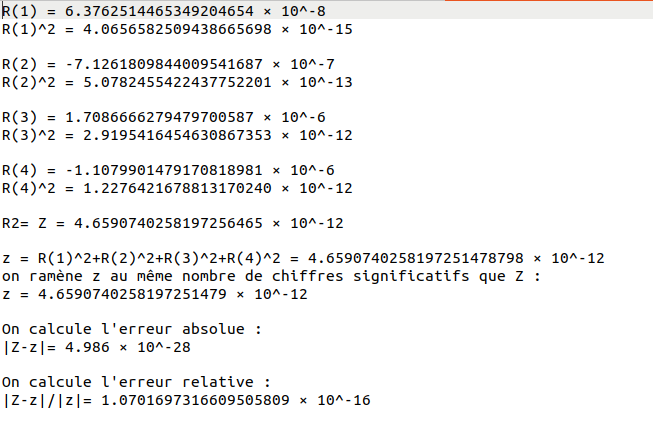
\includegraphics[width=0.9\textwidth]{./Images/r_3_err}
	\caption{Fichier d'erreur à l'étape 3}
\end{figure}

Encore on a une baisse de l'erreur absolue $10^{-28}$ mais l'erreur relative a tendance à remonter légèrement mais elle reste très faible.

\section{Etape 4}

\begin{figure}[H]
	\center
	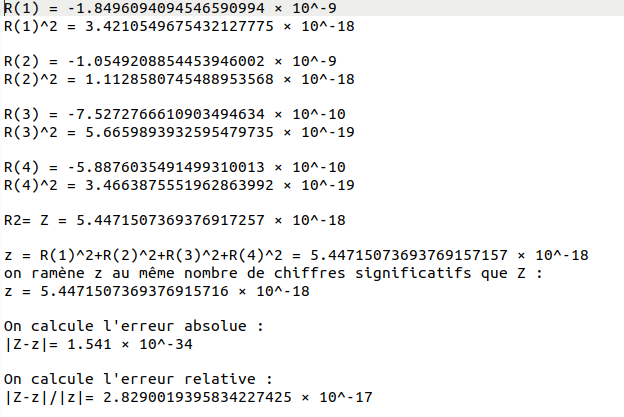
\includegraphics[width=0.9\textwidth]{./Images/r_4_err}
	\caption{Fichier d'erreur à l'étape 4}
\end{figure}

Encore une fois on a l'erreur absolue $10^{-32}$ qui diminue mais l'erreur relative reste aux alentours de $10^{-17}$ comme depuis le début.

\section{postambule}

On a pu voir que l'erreur absolue avait tendance à diminuer et l'erreur relative à stagner autour de $10^{-17}$. Il est en fait logique que l'erreur absolue diminue car le vecteur résidu diminue à chaque itération du programme normalement. C'est pourquoi il est souvent plus judicieux de regarder l'erreur relative qui est plus représentative.\\
A ce propos elle est plutôt très faible et on peut être satisfait du résultat obtenue.

\chapter{Vecteur solution $x$} %kev

\section{Etape 1}

\section{Etape 2}

\section{Etape 3}

\section{Etape 4}

\chapter{Analyse numérique du problème} %kev

Analysons maintenant le problème numériquement. On sait que la solution théorique est
$$x^T=\left(\begin{array}{cccc}
1 & 1 & 1 & 1\end{array}\right)$$

Comparons maintenant ce résultat avec celui qu'on a obtenu numériquement au bout de la $4^{eme}$ étape :
$$\hat{x}^T=\left(\begin{array}{cccc}
0.9999999987685677105 & 0.9999999992953791939 & 0.9999999994982825546 & 0.99999999960549057491\end{array}\right)$$\vspace{0cm}

On peut maintenant obtenir l'erreur absolue pour chaque composante afin d'obtenir le vecteur absolu :\footnote{calcul effectué sur \textit{wolframalpha.com}}

$$\varepsilon_{abs}=\left(\begin{array}{cccc}
1.2314322895*10^{-9} & 7.046208061*10^{-10} & 5.017174454*10^{-10} & 3.9450942509*10^{-10} \end{array}\right)$$\vspace{0cm}

On remarque que l'on obtient le même vecteur pour le vecteur erreur relative puisqu'on divise toutes les composantes par 1 :

$$\varepsilon_{rel}=\left(\begin{array}{cccc}
1.2314322895*10^{-9} & 7.046208061*10^{-10} & 5.017174454*10^{-10} & 3.9450942509*10^{-10} \end{array}\right)$$

On observe des erreurs beaucoup plus élevées que celles obtenues localement. En effet pour une étude local on obtenait des erreurs d'ordre de grandeur d'environ $10^{-17}$ alors qu'ici il est d'environ $10^{-10}$. Une différence de $10^{7}$ qui n'est pas négligeable.\\

Cependant, on peut souligner l'efficacité de la méthode car en seulement 4 itérations l'erreur de la solution obtenue par rapport à celle théorique est de seulement $10^{-9}$. Si l'on veut obtenir plus de précision il suffit de diminuer la tolérance et d'observer davantage d'étapes.





\chapter*{Conclusion} %thib
\addcontentsline{toc}{chapter}{Conclusion}

\chapter*{Annexe}

\end{document}
